% Template for CAD in medical imaging - Project Report
%          spconf.sty  - ICASSP/ICIP LaTeX style file, and
%          IEEEbib.bst - IEEE bibliography style file.
% --------------------------------------------------------------------------
\documentclass{article}
\usepackage{spconf,amsmath,graphicx}
\usepackage{subfigure}

% Title
\title{Computer Aided Diagnosis\\LUNA16: Candidate detection}
%
\makeatletter
\def\@name{ \emph{Luc Nies (s4136748)}, \emph{Tom van de Poll (s4106512)}, \emph{Harmen Prins (s4132297)}, \\ \emph{Steven Reitsma (s4132343)} \& \emph{Inez Wijnands (s4149696)}}
\makeatother

\address{Radboud University Nijmegen}
%
% For example:
% ------------
%\address{School\\
%	Department\\
%	Address}
%
% Two addresses (uncomment and modify for two-address case).
% ----------------------------------------------------------
%\twoauthors
%  {A. Author-one, B. Author-two\sthanks{Thanks to XYZ agency for funding.}}
%	{School A-B\\
%	Department A-B\\
%	Address A-B}
%  {C. Author-three, D. Author-four\sthanks{The fourth author performed the work
%	while at ...}}
%	{School C-D\\
%	Department C-D\\
%	Address C-D}
%
% More than two addresses
% -----------------------
% \name{Author Name$^{\star \dagger}$ \qquad Author Name$^{\star}$ \qquad Author Name$^{\dagger}$}
%
% \address{$^{\star}$ Affiliation Number One \\
%     $^{\dagger}$}Affiliation Number Two
%
\begin{document}
%\ninept
%
\maketitle
%
\begin{abstract}
Write your abstract here.
\end{abstract}


% Introduction
\section{Introduction}
\label{sec:intro}
In the \emph{LUng Nodule Analysis 2016 (LUNA16)} challenge, we aim to detect lung nodules in low-dose lung CT images. Firstly, we have segmented the lungs from the images. The next step is identifying candidates for lung nodules. Our aim is to detect enough candidates to include all actual lung nodules. In other words, be as sensitive as possible. The future step is of course to remove the false positives, but first we strive towards including the annotated nodules.

We continued working on the deep learning approach we used for the previous phase. In that phase we worked on lung segmentation and for this phase we treated candidate detection again as a segmentation problem. Secondly, we also used an image processing approach where we use the features of nodules such as blobness for candidate detection. These approaches and results are explained more detailed in the following sections.

% Table
\begin{table}[h]
\caption{\small{Caption here.}}
\label{tab:parameters}
\centering
\begin{tabular}{c | c | l}
text & text & text\\
\hline \hline
text & text & text
\end{tabular}
\end{table}

You can include figures as follows:

% Figure
\begin{figure}[h]
\centering
\subfigure[]
{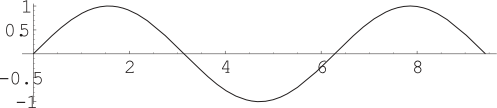
\includegraphics[width=0.7\linewidth]{./figure.png}}
\subfigure[]
{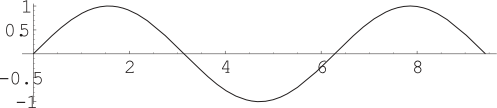
\includegraphics[width=0.7\linewidth]{./figure.png}}
\caption{Caption here. \label{figure:patterns}}
\end{figure}

% Method
\section{Method}\label{sec:method}
Explain the proposed method here.
You can use subsections to detail each part of your approach as follows. 
\subsection{Fully convolutional network}
Your text here.

\subsection{Blob detection}


% Experiments
%\section{Experiments}\label{sec:experiments}


% Results
\section{Results}\label{sec:results}


% Discussion
\section{Discussion}\label{sec:discussion}





% References should be produced using the bibtex program from suitable
% BiBTeX files (here: strings, refs, manuals). The IEEEbib.bst bibliography
% style file from IEEE produces unsorted bibliography list.
% -------------------------------------------------------------------------
\bibliographystyle{IEEEbib}

\begin{thebibliography}{}

\bibitem{ref1}
Authors, Year, Title, Journal, Volume, Pages.

\end{thebibliography}


\end{document}
